\documentclass[hidelinks, 12pt, a4paper]{article}

\usepackage[utf8]{inputenc}
\usepackage[margin=1.5cm]{geometry}
\usepackage{graphicx}
\usepackage{setspace}
\usepackage[T1]{fontenc}
\usepackage{tocloft}
\usepackage{todonotes}
\usepackage{epstopdf} 
\usepackage{hyperref}
\usepackage{float}
\usepackage{titlesec}
\usepackage{listings}
\usepackage{multirow}
\usepackage{xcolor}
\usepackage{mwe}
\usepackage{hyperref}
\onehalfspacing
\usepackage[english]{babel}
\usepackage{fancyhdr}
\usepackage{enumitem}

\pagestyle{fancy}
\fancyhf{}
\rhead{blulancetech@gmail.com}
\lhead{Carpool}
\rfoot{Page \thepage}

\author{}
\date{}
\title
{
	\includegraphics[width=6cm]{images/up_logo.jpg} \\
	Department of Computer Science \\
	Faculty of Engineering, Built Environment \& IT\\
	University of Pretoria \\
	\vspace{0.5cm}
	\Huge COS301 -
	Software Engineering\\
	\vspace{1cm}
	{\Huge Carpool}\\
	\begin{Large}
	Architectural requirements document
	\end{Large}
	\vspace{0.5cm}
	
    \begin{center}
    \noindent
    \includegraphics[width=6cm]{images/company_logo.png} 
    \vspace{0.5cm}
    \begin{table}[h]
    \centering
    \begin{tabular}{|l|l|l|}
    \hline
    Name  & Student Number\\ \hline
    Benjamin Osmers & u16068344 \\ \hline
    Ashleigh Govender &  U20528834      \\ \hline
    Jason Antalis     & U19141859     \\ \hline
    Wesley Pachai & U20578688    \\ \hline
            
    \end{tabular}
    \end{table}
    \end{center}
    }

\begin{document}
\maketitle


\newpage
\tableofcontents
\newpage
\section{Architectural design strategy}
The architectural design strategy employed during the development of carpool  is  composed of two methods: decomposition and the consideration of quality requirements.
\newline \\
When implementing the decomposition strategy, we split the system up into smaller subsystems namely: client-side, back-end, and database systems. By splitting the system up into smaller subsystems, it makes it easier to work with the system as well as update the system. Suitable architectural designs were considered based on each subsystem.
\newline \\
These designs were then narrowed down based on the quality requirements that are listed below. Using quality requirements to design our system ensures that our system meets the necessary standards and performs the way we want it to.
\vspace{0.75cm}
\section{Architectural design styles}
Our system is comprised of four different Architectural design styles which are all combined together. The four styles are:

\subsection{\textbf{Client-server Pattern:}}
\newline
Since the carpool application relies heavily on user input (users will be querying the database on a regular basis), the logic and data storage needs to be separate from the mobile application. The client in this case will be the mobile application whilst the server is the database and logic of the system. The system will consist of users (both drivers and passengers) all of which need to connect to the server when using the carpool application. The database is responsible for storing information about drivers, passengers, and trips.
The client-server pattern was used as many clients request and receive service from a centralized database (server) \\ \\
This style allows us to achieve security as the server can have checks which prevent unauthenticated clients from sending request.\\ \\
This style allows us to achieve useability, since the mobile application is separate from the logic and data storage of the system, the user is not concerned with the underlining functionality of the system. The user only has to worry about the front-end.

\begin{center}
    \noindent
    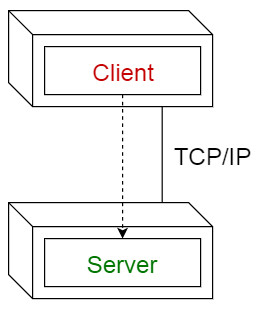
\includegraphics[width=4cm]{images/client_server.png}
    \vspace{0.5cm}
\end{center}
\subsection{\textbf{Model View Controller:}}
\newline
Since the carpool applications needs to perform CRUD operations on  the database, the Model View Controller pattern will be used. The model is responsible for handling the data logic, it is connected to the database. The view helps to represent the data(from the model) in a way that is easily read-able to the user. The controller functions as a middleman between the views and the model by allowing them to communicate with each other.
The layout of the application follows the layout of the model view controller pattern, for example: the passanger will have to be able to view available trips (view -> controller -> model).
The Model view Controller was used as it facilitates the development of a dynamic and reactive front-end  \\ \\
This style allows us to achieve Maintainability. Since the model view controller provides modularity, one is able easily upgrade/ change the system without hassle  .\\ \\
This style allows us to achieve useability, because of the architecture's separation of concerns, it has the potential to ease user interface development.
 \vspace{0.2cm}
\begin{center}
    \noindent
    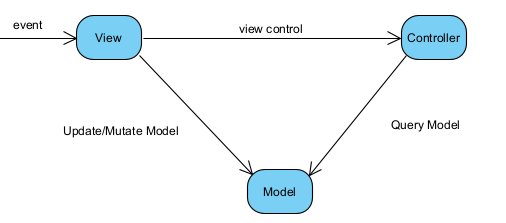
\includegraphics[width=10cm]{images/model_view_controller.png}
    \vspace{0.5cm}
\end{center}
\subsection{\textbf{Layered:}}
\newline
The application will make use of the layered pattern. The pattern facilities communication between the back-end and front-end of the carpool application. The system will be broken up into many different layers, which will allow us to modify, maintain and expand the application easily.
The layered pattern was used as it uses a control layer to facilitate the separation of concerns and security. \\ \\
This style allows us to achieve scalability, since the system can be broken up into layers, adding more functionality to the system simply means adding another layer to the system (or components to a specific layer), which can be done easily as the layers are independent of each other. The layers that our system will be broken up into are: Application, Presentation, Logic and Database layer.\\ \\
Application: Handles all of the logic that the application need to meet its functional requirements.
Presentation: Where the user interface component is included. Model View Controller patterns sits on this layer.
Logic: Handles the data and performs the necessary functions on the data.
Database: All aspects relating to the database
This style allows us to achieve reliability since the pattern divides possible points of failure into loosely linked layers.
\begin{center}
    \noindent
    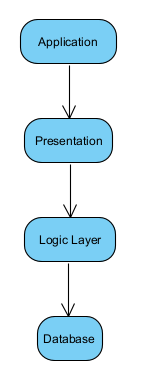
\includegraphics[width=4cm]{images/layered.png}
    \vspace{0.5cm}
\end{center}
\subsection{\textbf{REST:}}
\newline
The REST (Representational State Transfer) architectural style will be used for data transit. A loosely linked application can be created with the REST approach. For transportation, the REST style will work well with our other Client Server Style.
% \begin{center}
%     \noindent
%     \includegraphics[width=10cm]{images/.png}
%     \vspace{0.5cm}
% \end{center}
\subsection{\textbf{Conclusion:}}
The application makes use of the client-side pattern, within this client-side pattern, the layered pattern is used to facilitate communication between the back-end and front end of the carpool system. The model view controller is used on the presentation layer to assist with the querying of the database. And REST will be used to transport the data.
\newpage
\section{Architectural Quality requirements}
\large{\textbf{Usability:}}
\begin{itemize}[]
            \item [-]The user should be able to see the system's responses, whether favorable or negative. These responses should contain enough information, allowing the user to know exactly what went wrong or right.
            \item [-]Buttons, graphics, and text should be made large enough to improve clarity, user comfort, reduce annoyance, and reduce the chance of selection mistakes.
        \end{itemize}
\vspace{0.5cm}
\large{ \textbf{Scalability}}
\begin{itemize}
      \item[-]Currently the carpool application is only for students in South Africa but it could be expanded internationally. As the number of users and operations grows, the server and database must be able to scale both vertically and horizontally.  The system must be able to accommodate a user base from 100 users to 1 million users.
\end{itemize}
\vspace{0.5cm}
\large{ \textbf{Availability}}
\begin{itemize}
      \item[-] The system is expected to have at least 99.5\% uptime.This app should be available to all users, at all times of the day. For example, if a driver wants to post a ride at the middle of night and a passenger wants to book a ride at the same time then the system should be able to handle this.
\end{itemize}
\vspace{0.5cm}
\large{ \textbf{Reliability:}}
\begin{itemize}
        \item[-] The system should be operational 99.9\% of the time.
      \item[-] The software should be extremely reliable. If a crash occurs, the system should be able to offer sufficient information as to why the crash happened, allowing us to swiftly correct the problem.
\end{itemize}
\newpage
\large{ \textbf{Maintainability}}
\begin{itemize}
      \item[-] The system should be checked and maintained on a regular basis, at least twice a month. Users should be informed about this maintenance at least 24 hours ahead of time so that they may make the required preparations.
      \item [-] It should be simple to add new functionality to the system or alter existing functionality. The system should be decoupled as much as possible. We should be certain that the technology we choose will be supported for a long time.
      \end{itemize}
\vspace{0.5cm}
\large{ \textbf{Performance}}
\begin{itemize}
      \item[-] Reading is more significant than writing since users are more likely to spend time browsing than posting trips. As a result, few actions write to the database. Hence a read operation should take less than 500ms and a write operation should approximately 1s.
\end{itemize}
\vspace{0.5cm}
\large{ \textbf{Security}}
\begin{itemize}
      \item [-] Because users' passwords and banking details  are kept in the database, the database must be encrypted or hashed in order to safeguard this data.
      \item [-] Every user has their own unique username and password, which ensures that unauthorised users do not have access to the database.
\end{itemize}
\newpage
\section{Architectural design and patterns}
\begin{center}
    \noindent
    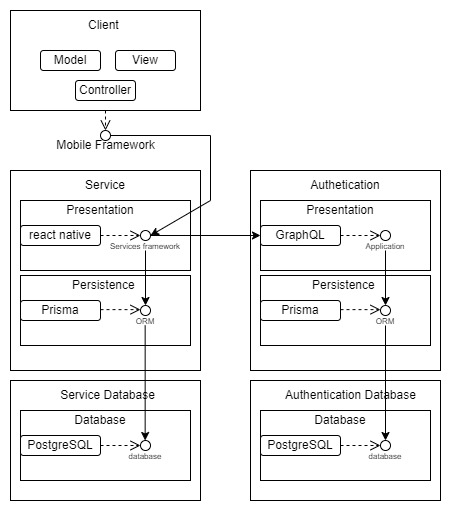
\includegraphics[]{images/Architecture301_1.jpg}
    \vspace{0.5cm}
\end{center}

\newpage
\section{Architectural constraints}
The architectural constraints of Carpool are few and hence would not impose much of a limit on the system. These constraints are as follows:\\
•    The system must be deployable to mobile devices.\\
•    Must be deployable to both Android and iOS.\\
•    The backend must run remotely.\\
\section{Technology Choices}
\subsection{Front-End}
The chosen front-end technology is React Native along side redux.
React Native allows us to create mobile applications using website technology and create cross-platform mobile applications, Android and iOS for example.
It allows faster development since the apps do not need to be recompiled but rather the app can be reloaded and the changes will be reflected on the device.
Flutter and Angular are also popular front-end technologies.
We opted for React Native since it provides accessibility to intelligent debugging tools and error reporting.
As well as, Flutter cannot create apps for android and Angular has lowered app performance when compared with React Native.
Unfortunately, React Native does not support parallel threading and multi-processing.
\newline
\newline
Looking at the candidates of redux, flux and mvc, we chose redux as it is a state management framework that is easy to use and easy to understand.
All of these candidates revolve around the Model View Controller pattern.
Rather than placing state information in multiple Stores across the application, Redux keeps everything in one region of the app.
\subsection{Back-End}
NestJS, GraphQL and the Prisma Client are all the choices for the back-end technologies.
Looking at our architecture, we chose NestJS as it is can be based on the Model View Controller pattern.
While ExpressJs does not follow the MVCPattern which our architecture is based on, it does not have as much structure as NestJs causing it to be inefficient.
On the API side, we chose GraphQL as it is a query language and REST is more of an architectural pattern/style.
Due to using the Prisma ORM, it is logical to therefore use the prisma client for our database needs.
\subsection{Database}
Database systems are used to store and retrieve data.
The two options were PostgreSQL and MySQL.
We opted for PostgreSQL since it has much more functionality than MySQL.
For example PostgreSQL allows us to create different data types for a specific array of data.
Another advantage over MySQL is that it is supports analytic functions.
\newline
\newline
Onto Object Relational Mapping (ORM) frameworks, we chose Prisma.
It makes database access easy with auto-generated query builder for TypeScript.
\subsection{Hosting}
When looking at hosting options, there many options which range from AWS, Azure and Google.
We chose Google Hosting because it is the most cost effective and it is also a popular option.
There is not a lot of difference between the various hosting services and generally comes down to preference.
\newpage
\end{document}